% =====================================================================================
% Supplemental Material. Compile separately (pdflatex + bibtex), or set it as the main
% document in Overleaf. Figures: run/fig_artigo.py; tables: run/tabelas_artigo.py.
% =====================================================================================
\documentclass[aps,pra,onecolumn,superscriptaddress,11pt,longbibliography,floatfix,nofootinbib]{revtex4-2}

\usepackage{graphicx}
\usepackage{amsmath,amssymb}
\usepackage{bm}
\usepackage{booktabs}
\usepackage{multirow}
\usepackage{xcolor}
\usepackage[colorlinks=true,linkcolor=blue!50!black,citecolor=blue!50!black,urlcolor=blue!50!black]{hyperref}

\graphicspath{{figures/}}

\newif\ifshowtodos \showtodostrue
\newcommand{\TODO}[1]{\ifshowtodos\textcolor{red}{\textbf{[TODO:} #1\textbf{]}}\fi}
\newcommand{\rvec}{\bm r}
\newcommand{\ef}{\epsilon_f}
\newcommand{\er}{\epsilon_r}

% S-numbering of sections, equations, figures and tables
\renewcommand{\thesection}{S\arabic{section}}
\renewcommand{\theequation}{S\arabic{equation}}
\renewcommand{\thefigure}{S\arabic{figure}}
\renewcommand{\thetable}{S\arabic{table}}

\begin{document}

\title{Supplemental Material for\\ ``Recovering a time-dependent control field from qubit expectation
values: physics-informed neural networks versus classical inversion''}

\author{Gubio G. de Lima}
\affiliation{Physics Department, Federal University of S\~ao Carlos, 13565-905, S\~ao Carlos, SP, Brazil}

\date{\today}

\maketitle

This document gives the technical details and all numerical values needed to reproduce the results of
the main text. Every number below is produced by the scripts of the code repository
(\url{https://github.com/GubioGL/Pinn-inverse-for-H-time}): \texttt{run/rodar.py} runs the benchmark,
\texttt{run/tabelas\_artigo.py} writes the tables and \texttt{run/fig\_artigo.py} the figures. Source
files are indicated as \texttt{src/<file>.py}.

\tableofcontents

% =====================================================================================
\section{Data generation and units}\label{sec:data}

\paragraph{Model and units.} The Hamiltonian is $H(t)=\tfrac12\sigma_z+\tfrac12f(t)\sigma_x$ with
$\hbar=1$ and unit qubit splitting; time is measured in units of the inverse splitting and the field
$f$ in units of the splitting. For a pure state, the Bloch vector $\rvec=(X,Y,Z)$ obeys
\begin{equation}
  \dot\rvec = \bm\Omega(t)\times\rvec,\qquad \bm\Omega=(f,0,1),
  \label{eq:S_bloch}
\end{equation}
which is equivalent to the Schr\"odinger (or von Neumann) equation for this Hamiltonian.

\paragraph{Test fields.} Table~\ref{tab:fields} lists the fields. Field~3 and the single-tone pulses of
the spectral study (\texttt{"w<omega>"} cases in \texttt{src/bloch.py}) share the envelope
$\sin^2(\pi t/T)$, so $f(0)=f(T)=0$; this is a property of the pulse design and is the only information
about the field used by the edge constraint of Sec.~\ref{sec:edges}.

\begin{table}[h]
  \caption{Test fields. All are evaluated on $N=100$ equally spaced times $t_i\in[0,T]$.}
  \label{tab:fields}
  \begin{tabular}{llcl}
    \toprule
    field & $f(t)$ & $T$ & remarks \\
    \midrule
    1 & $\cos t$ & $2\pi$ & periodic on $[0,T]$, single harmonic \\
    2 & $1.5\sin2t+0.8\cos(3.5t+0.5)+0.4\sin7t$ & $2.52\pi$ & $f(0)\ne f(T)$, not periodic \\
    3 & $[1.5\sin2t-0.3\cos(3t-0.5)+0.4\sin7t]\,\sin^2(\pi t/T)$ & $2.52\pi$ & smooth pulse, $f(0)=f(T)=0$ \\
    $\omega$ & $\sin(\omega t)\,\sin^2(\pi t/T)$ & $2.52\pi$ & spectral study, $\omega\in\{1,\dots,20\}$ \\
    \bottomrule
  \end{tabular}
\end{table}

\paragraph{Integration.} Equation~\eqref{eq:S_bloch} is integrated with the eighth-order
Dormand--Prince method (SciPy \texttt{solve\_ivp}, method \texttt{DOP853}) with relative tolerance
$10^{-11}$ and absolute tolerance $10^{-12}$ (\texttt{src/bloch.py::simulate}). As a cross-check, the
same trajectories obtained with QuTiP \texttt{mesolve}~\cite{johansson2013qutip} differ by less than
$5\times10^{-11}$ when the field is passed as a function, and by $8\times10^{-6}$ when it is passed as an
array sampled at the data times (QuTiP then interpolates it with cubic splines).

\paragraph{Noise.} Noisy data are $\rvec_i=\rvec(t_i)+\bm\eta_i$ with independent Gaussian components of
standard deviation $\sigma\in\{0,0.01,0.03\}$. For reference, $\sigma=0.01$ corresponds to the
projection noise of $\sim\!10^4$ single-shot measurements per expectation value.

\paragraph{Seeds.} For each (field, $\sigma$, seed $s$) the data are generated once, with the random
generator seeded by $10^5c+10^3\lfloor10^3\sigma\rceil+s$, where $c$ is the field index
(\texttt{src/executar.py::gerar\_dados}). All methods receive the same data. The seed $s\in\{0,\dots,4\}$
also sets the initialization of every network and the random collocation points.

% =====================================================================================
\section{Identifiability}\label{sec:identifiability}

\paragraph{Pointwise inversion and sensitivity.} The second and third components of
Eq.~\eqref{eq:S_bloch} read $fZ=X-\dot Y$ and $fY=\dot Z$. Minimizing $(fZ-X+\dot Y)^2+(fY-\dot Z)^2$
over $f$ at each instant gives
\begin{equation}
  f = \frac{Z(X-\dot Y)+Y\dot Z}{Y^2+Z^2}.
  \label{eq:S_direct}
\end{equation}
The derivative of the right-hand side of Eq.~\eqref{eq:S_bloch} with respect to $f$ is
$(0,-Z,Y)$, whose squared norm $Y^2+Z^2=1-X^2$ measures the local sensitivity of the dynamics to the
field. It vanishes when the Bloch vector is parallel to the control axis. For the initial state
$|+\rangle$ it vanishes at $t=0$; Table~\ref{tab:observ} quantifies this for the three test fields.

\begin{table}[h]
  \caption{Fraction of the interval in which $Y^2+Z^2<0.05$, and minimum of $Y^2+Z^2$, for three
  initial states (computed on 400 equally spaced times; \texttt{run/diagnostico.py}).}
  \label{tab:observ}
  \begin{tabular}{lcccccc}
    \toprule
    & \multicolumn{2}{c}{$|+\rangle$} & \multicolumn{2}{c}{$|0\rangle$} & \multicolumn{2}{c}{$(1,1,1)/\sqrt3$} \\
    \cmidrule(lr){2-3}\cmidrule(lr){4-5}\cmidrule(lr){6-7}
    field & fraction & minimum & fraction & minimum & fraction & minimum \\
    \midrule
    1 & 9.0\% & 0 & 0\% & 0.38 & 6.0\% & 0.018 \\
    2 & 7.0\% & 0 & 0\% & 0.13 & 0\% & 0.26 \\
    3 & 4.0\% & 0 & 0\% & 0.52 & 5.2\% & 0.011 \\
    \bottomrule
  \end{tabular}
\end{table}

\paragraph{Initial state and measurement budget.} Table~\ref{tab:initial} compares designs with the same
total number of measurements: splitting the budget over more time points or more initial states
increases the noise per point by $\sqrt{\text{(number of points)}/100}$. Preparing $|0\rangle$ instead of
$|+\rangle$ halves the error of linear least squares and reduces its spread over noise realizations by a
factor of six; three initial states perform like $|0\rangle$ with LSQ and better with shooting at the
higher noise level.

\begin{table}[h]
  \caption{Field~3: relative field error (mean $\pm$ standard deviation over five noise realizations) for
  designs with the same measurement budget; $\sigma_{\rm ref}$ is the noise of the reference design (one
  state, $N=100$). Linear least squares with 40 cubic B-splines and shooting initialized by it
  (\texttt{run/parte1\_classicos.py}).}
  \label{tab:initial}
  \begin{tabular}{lccccc}
\toprule
design & $\sigma$ per point & \multicolumn{2}{c}{$\sigma_{\rm ref}=0.01$} & \multicolumn{2}{c}{$\sigma_{\rm ref}=0.03$} \\
\cmidrule(lr){3-4}\cmidrule(lr){5-6}
 & & LSQ & shooting & LSQ & shooting \\
\midrule
$|+\rangle$, $N=100$ & $\sigma$ & $0.153\pm0.053$ & $0.093\pm0.010$ & $0.311\pm0.151$ & $0.225\pm0.018$ \\
$|0\rangle$, $N=100$ & $\sigma$ & $0.069\pm0.008$ & $0.067\pm0.005$ & $0.151\pm0.024$ & $0.194\pm0.012$ \\
$|+\rangle$, $N=300$ & $\sqrt{3}\,\sigma$ & $0.190\pm0.062$ & $0.073\pm0.009$ & $0.245\pm0.087$ & $0.198\pm0.027$ \\
$|+\rangle,|0\rangle,|{+i}\rangle$, $N=100$ each & $\sqrt{3}\,\sigma$ & $0.073\pm0.012$ & $0.069\pm0.015$ & $0.158\pm0.021$ & $0.151\pm0.031$ \\
\bottomrule
\end{tabular}

\end{table}

\paragraph{Symmetries.} Two symmetries of Eq.~\eqref{eq:S_bloch} map a solution for $f$ onto a solution
for $-f$:
\begin{align}
  (X,Y,Z,f)&\to(-X,-Y,Z,-f), & &\text{(rotation by $\pi$ about $z$; $\sigma_zH(f)\sigma_z=H(-f)$)},\\
  (X,Y,Z,f)&\to(X,Y,-Z,-f). & &
\end{align}
The first leaves invariant the initial states with $X=Y=0$ ($|0\rangle$, $|1\rangle$) and preserves
$Z(t)$; the second leaves invariant the initial states with $Z=0$ (e.g.\ $|+\rangle$) and preserves
$X(t)$ and $Y(t)$. Consequently, the sign of $f$ cannot be recovered from $\langle\sigma_z\rangle$ alone
when starting from $|0\rangle$, nor from $\langle\sigma_x\rangle$ and $\langle\sigma_y\rangle$ when
starting from $|+\rangle$. Numerically, for the three test fields the invariant components agree to
machine precision, while the others differ by $0.9$--$2$; for the generic state $(1,1,1)/\sqrt3$ all
components differ by $0.8$--$1.5$.

\paragraph{Sensitivity to the frequency of the field.} Figure~\ref{fig:S1} shows the RMS change of the
data produced by a perturbation $a\sin(\omega t)\sin^2(\pi t/T)$ of field~3, per unit $a$, as a function
of $\omega$ (finite differences with $a=10^{-4}$). The decay is close to $1/\omega$: the forward map
integrates the field, so high frequencies are weakly encoded in the data.

\begin{figure}[h]
  \centering
  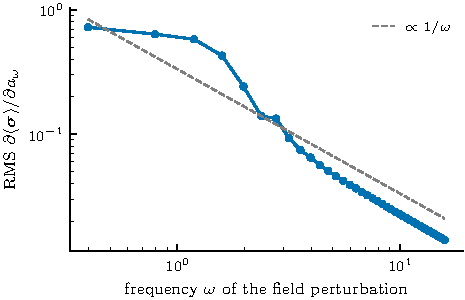
\includegraphics[width=0.48\linewidth]{figS1_sensitivity.pdf}
  \caption{Sensitivity of the data to a perturbation of frequency $\omega$ of field~3 (initial state
  $|0\rangle$).}
  \label{fig:S1}
\end{figure}

% =====================================================================================
\section{Field representations}\label{sec:representations}

\paragraph{Fourier series} ($M=10$, 21 coefficients):
\begin{equation}
  f(t)=a_0+\sum_{m=1}^{M}\big[a_m\cos(2\pi mt/T)+b_m\sin(2\pi mt/T)\big],
\end{equation}
with highest angular frequency $2\pi M/T=7.9$.

\paragraph{Cosine series} ($M=40$, 41 coefficients): $f(t)=\sum_{m=0}^{M}c_m\cos(m\pi t/T)$, the even
extension of $f$ to period $2T$. Highest angular frequency $\pi M/T=15.9$.

\paragraph{Cubic B-splines} ($n=80$, $k=3$): $f(t)=\sum_{j=1}^{n}c_jB_{j,3}(t)$ on the open uniform knot
vector with $k+1=4$ repeated knots at each end and $n-k-1=76$ equally spaced interior knots (spacing
$h=T/77=0.103$ for $T=2.52\pi$). The basis is evaluated by the Cox--de Boor
recursion~\cite{deboor2001splines}, implemented in PyTorch (\texttt{src/pinn.py::bspline\_torch}); it
agrees with SciPy's \texttt{BSpline.design\_matrix} to $2\times10^{-10}$. The original notebooks used
degree $k=10$ with $n=30$, which is less accurate for the same number of coefficients (Fig.~\ref{fig:S2}).

\paragraph{Neural-network field.} An extra (fourth) output of the state network
(Sec.~\ref{sec:pinn}); 33 additional parameters.

\paragraph{MixFunn.} Two MixFunn layers~\cite{farias2025mixfunn} ($1\to4\to1$ neurons) with the function
dictionary $\{\sin x,\cos x,e^{-0.01|x|},x\}$ and second-order neurons (products of pairs of dictionary
functions, $4\cdot5/2=10$ products), i.e.\ $4+10=14$ mixing weights per neuron; 274 parameters in total.
The input is the raw time $t$ in the Adam-only recipe (as in the original code) and the normalized time
$s$ in the improved recipes. Mixing weights are initialized from a standard normal distribution and the
linear projections with PyTorch's default initialization.

\paragraph{Capacity of the bases.} Figure~\ref{fig:S2} shows the best $L_2$ approximation error of
single-tone pulses $\sin(\omega t)\sin^2(\pi t/T)$ by each basis. The Fourier basis with $M=10$ cannot
represent frequencies above $7.9$; cubic B-splines with $n=80$ functions represent the pulses with
error below $10^{-2}$ up to $\omega\approx15$. For the test fields, the best-approximation errors of
field~2 are $0.14$ (Fourier, $M=10$), $1.1\times10^{-2}$ (cosine, $M=40$) and $6.9\times10^{-5}$ (B-spline,
$n=80$); for field~3 they are $4.9\times10^{-3}$, $7.0\times10^{-5}$ and $8.5\times10^{-5}$, respectively.

\begin{figure}[h]
  \centering
  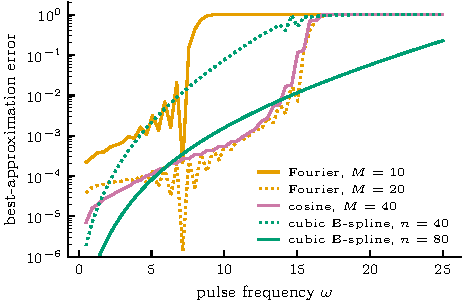
\includegraphics[width=0.48\linewidth]{figS2_bases.pdf}
  \caption{Best-approximation error of single-tone pulses by each field basis.}
  \label{fig:S2}
\end{figure}

\paragraph{Edge constraint.}\label{sec:edges} When $a=f(0)$ and $b=f(T)$ are known, every representation
$g$ is replaced by
\begin{equation}
  f(t) = g(t) - (1-\tau)\,g(0) - \tau\,g(T) + (1-\tau)\,a + \tau\,b,\qquad \tau=t/T,
\end{equation}
which satisfies $f(0)=a$ and $f(T)=b$ exactly and is linear in $g$. For the bases, $f=\tilde{\mathsf B}\bm c
+\bm m$ with $\tilde B_{j}(t)=B_j(t)-(1-\tau)B_j(0)-\tau B_j(T)$ and $m(t)=(1-\tau)a+\tau b$. The constraint
is applied only to field~3 and to the spectral pulses ($a=b=0$).

\begin{table}[h]
  \caption{Number of trainable parameters: field only, and total (state network plus field) for the two
  network architectures (Table~\ref{tab:hyper}).}
  \label{tab:params}
  \begin{tabular}{lccc}
    \toprule
    representation & field & total, Adam-only recipe & total, improved recipes \\
    \midrule
    NN field & 16 / 33 & 334 & 2308 \\
    Fourier ($M=10$) & 21 & 339 & 2296 \\
    cosine ($M=40$) & 41 & 359 & 2316 \\
    B-spline ($n=80$) & 80 & 398 & 2355 \\
    MixFunn & 274 & 592 & 2549 \\
    \bottomrule
  \end{tabular}
\end{table}

% =====================================================================================
\section{Physics-informed neural network}\label{sec:pinn}

\paragraph{State network.} A fully connected network with $L$ hidden layers of width $W$ and sine
activations maps the input to three outputs (four when the field is a network output). Weights and
biases of each layer are drawn from $\mathcal U(-1/\sqrt{n_{\rm in}},1/\sqrt{n_{\rm in}})$, where
$n_{\rm in}$ is the input width of the layer (PyTorch's default). Improved recipes: $L=3$, $W=32$,
input $s=2t/T-1$, double precision. Adam-only recipe: $L=2$, $W=15$, input $t$, single precision.

\paragraph{Initial condition.} Improved recipes impose $\rvec(0)=\rvec_0$ exactly,
\begin{equation}
  \rvec_{\bm\theta}(t)=\rvec_0+\frac{t}{T}\,\mathcal N_{\bm\theta}(s),\qquad
  \dot\rvec_{\bm\theta}(t)=\frac{1}{T}\mathcal N_{\bm\theta}(s)+\frac{t}{T}\frac{2}{T}\,\mathcal N'_{\bm\theta}(s).
\end{equation}
The Adam-only recipe has no such constraint; the initial condition enters only through the data point at
$t=0$.

\paragraph{Time derivative.} For a layer $\bm h_{l+1}=\sin(\mathsf W_l\bm h_l+\bm b_l)$, the time
derivative is propagated together with the activations,
$\dot{\bm h}_{l+1}=\cos(\mathsf W_l\bm h_l+\bm b_l)\odot\mathsf W_l\dot{\bm h}_l$, starting from
$\dot{\bm h}_0=ds/dt=2/T$. This forward-mode derivative is exact (it agrees with reverse-mode automatic
differentiation to $10^{-17}$) and requires a single pass, whereas the usual approach differentiates the
network output with respect to its input by a backward pass that must itself be differentiated during
training.

\paragraph{Loss and residual vector.} With collocation set $\mathcal C$, the loss is
\begin{equation}
  \mathcal L = \frac{1}{|\mathcal C|}\sum_{t\in\mathcal C}\|\bm R(t)\|^2
  + \frac{w}{N}\sum_{i=1}^{N}\|\rvec_{\bm\theta}(t_i)-\rvec_i\|^2
  + \frac{\lambda_f h_r}{T}\sum_{k=2}^{n_r-1}\Big(\frac{f_{k+1}-2f_k+f_{k-1}}{h_r^2}\Big)^2,
  \label{eq:S_loss}
\end{equation}
where $\bm R=\dot\rvec_{\bm\theta}-\bm\Omega_{\bm\theta}\times\rvec_{\bm\theta}$, $w=1$, and $f_k$ is the
field on a fixed uniform grid of $n_r=200$ points with spacing $h_r$; the last term approximates
$(\lambda_f/T)\int f''^2dt$. Equation~\eqref{eq:S_loss} is exactly $\|\bm\rho\|^2$ for the residual vector
$\bm\rho$ obtained by stacking $\bm R(t)/\sqrt{|\mathcal C|}$, $\sqrt{w/N}(\rvec_{\bm\theta}(t_i)-\rvec_i)$
and the scaled second differences. Its length is $3|\mathcal C|+3N$ ($+\,n_r-2$ with noise); with
$|\mathcal C|=300$ and $N=100$, $\dim\bm\rho=1200$ without noise.

\paragraph{Collocation.} $\mathcal C$ contains the $N$ data times and $n_{\rm rand}=200$ times drawn
uniformly in $[0,T]$, redrawn at every Adam epoch (3000 draws, i.e.\ $6\times10^5$ distinct points).
L-BFGS, BFGS and LM require a fixed objective during the line search or the trust-region test and use
the last draw; LM can optionally redraw every $K$ iterations. The Adam-only recipe uses the data times
only.

\paragraph{Smoothness weight.} $\lambda_f$ is fixed a priori by the noise level:
$\lambda_f=0$ ($\sigma=0$), $10^{-6}$ ($\sigma=0.01$) and $10^{-5}$ ($\sigma=0.03$). These values
correspond to the coefficient penalty of the classical LSQ estimator (Sec.~\ref{sec:classical}),
$\lambda_f\approx\lambda_{D}h^3T/N$ for knot spacing $h$.

\paragraph{Least-squares initialization and variable projection.} For a linear representation
$f=\tilde{\mathsf B}\bm c+\bm m$ and given $(X,Y,Z,\dot Y,\dot Z)$ at $n$ points, the part of
Eq.~\eqref{eq:S_loss} that depends on $\bm c$ is quadratic, and its minimizer solves
\begin{equation}
  \Big[\tfrac1n\tilde{\mathsf B}^{\top}\mathrm{diag}(Y^2+Z^2)\tilde{\mathsf B}
       +s^2(\mathsf D_2\tilde{\mathsf B}_r)^{\top}\mathsf D_2\tilde{\mathsf B}_r\Big]\bm c
  = -\tfrac1n\tilde{\mathsf B}^{\top}\big[Z(\dot Y-X+mZ)-Y(\dot Z-mY)\big]
    -s^2(\mathsf D_2\tilde{\mathsf B}_r)^{\top}\mathsf D_2\bm m_r ,
\end{equation}
with $s^2=\lambda_fh_r/T$, $\mathsf D_2$ the second-difference matrix divided by $h_r^2$, and
$\tilde{\mathsf B}_r$, $\bm m_r$ the basis and offset on the regularization grid.
The \emph{initialization} uses the data and their cubic-spline derivatives (smoothing spline with
generalized cross-validation for noisy data); \emph{variable projection}~\cite{golub1973varpro} uses the
current network state at the collocation points at every Adam epoch.

\paragraph{Optional terms.} Causal weights~\cite{wang2022causality}: the collocation points are sorted
in time and split into 20 blocks with mean residuals $\mathcal L_k$; block $k$ is weighted by
$\exp(-\epsilon\sum_{j<k}\mathcal L_j)$ with $\epsilon=1$ (weights not differentiated). Gradient-norm
balancing~\cite{wang2021gradient}: every 100 Adam epochs,
$w\leftarrow(1-\alpha)w+\alpha\max|\nabla\mathcal L_{\rm ODE}|/\overline{|\nabla\mathcal L_{\rm data}|}$
with $\alpha=0.1$; $w$ is reset to 1 after Adam so that the second stage minimizes the same objective
for all methods.

% =====================================================================================
\section{Optimizers}\label{sec:optimizers}

All optimizers act on a single flat parameter vector (network and field). Table~\ref{tab:hyper}
summarizes the recipes; details follow.

\begin{table}[h]
  \caption{Training recipes (generated from \texttt{src/protocolo.py}).}
  \label{tab:hyper}
  \begin{tabular}{p{0.2\linewidth}p{0.34\linewidth}p{0.38\linewidth}}
\toprule
item & Adam-only recipe (as in common practice) & improved recipes \\
\midrule
state network & $2$ hidden layers $\times$ $15$, $\sin$ & $3$ hidden layers $\times$ $32$, $\sin$ \\
network input & $t$ & $s=2t/T-1$ \\
initial condition & soft (data term) & hard, $\boldsymbol r(t)=\boldsymbol r_0+(t/T)\,\mathrm{NN}$ \\
field edges & free & hard when known ($f(0)=f(T)=0$ for field 3) \\
collocation points & the $N=100$ data points & $N$ data points $+$ $200$ uniform random points, redrawn every Adam epoch \\
field coefficients at start & zero & linear least squares on the data \\
floating point & single (float32) & double (float64) \\
Adam & 20000 epochs, learning rate $1\times10^{-3}$, constant & 3000 epochs, learning rate $1\times10^{-3}$ $\to$ $1\times10^{-5}$ (cosine schedule) \\
second stage & none & L-BFGS 5000 it.\ (history 50, strong Wolfe); BFGS 8000 it.; LM 600 it. \\
smoothness weight $\lambda_f$ & \multicolumn{2}{l}{$\sigma=0$: $0$; $\sigma=0.01$: $1\times10^{-6}$; $\sigma=0.03$: $1\times10^{-5}$} \\
time limit per run & \multicolumn{2}{l}{420 s (single CPU thread)} \\
\bottomrule
\end{tabular}

\end{table}

\paragraph{Adam}~\cite{kingma2015adam} with $\beta_1=0.9$, $\beta_2=0.999$, $\epsilon=10^{-8}$. Improved
recipes: 3000 epochs, learning rate decaying from $10^{-3}$ to $10^{-5}$ with a cosine schedule.
Adam-only recipe: 20000 epochs at a constant learning rate $10^{-3}$.

\paragraph{L-BFGS}~\cite{liu1989lbfgs} (PyTorch implementation): unit initial step, history 50,
strong-Wolfe line search, at most 5000 iterations and 6250 function evaluations, gradient tolerance
$10^{-15}$, change tolerance $10^{-18}$.

\paragraph{Dense BFGS.} The inverse Hessian $\mathsf H$ is stored as a dense matrix. After the first
step, $\mathsf H$ is reset to $(\bm s^{\top}\bm y/\bm y^{\top}\bm y)\mathsf I$; every iteration uses a
strong-Wolfe line search (at most 30 evaluations) and the update
\begin{equation}
  \mathsf H\leftarrow\tau\Big[\mathsf H-\frac{\mathsf H\bm y\bm y^{\top}\mathsf H}{\bm y^{\top}\mathsf H\bm y}
  +(\bm y^{\top}\mathsf H\bm y)\,\bm v\bm v^{\top}\Big]+\frac{\bm s\bm s^{\top}}{\bm s^{\top}\bm y},\qquad
  \bm v=\frac{\bm s}{\bm s^{\top}\bm y}-\frac{\mathsf H\bm y}{\bm y^{\top}\mathsf H\bm y},
\end{equation}
with $\tau=1$ (BFGS) or $\tau=\min(1,\bm s^{\top}\bm y/\bm y^{\top}\mathsf H\bm y)$ (self-scaled variant,
in the spirit of Refs.~\cite{urban2025unveiling,kiyani2025optimizer}; it is not the exact SSBroyden
update of those works). $\mathsf H$ is reset after a failed line search, and the run stops after three
consecutive failures or 8000 iterations.

\paragraph{Levenberg--Marquardt}~\cite{levenberg1944,marquardt1963}. With $\mathsf J=\partial\bm\rho/
\partial\bm\theta$ ($R\times P$), the step is
$\delta\bm\theta=-(\mathsf J^{\top}\mathsf J+\mu\mathsf I)^{-1}\mathsf J^{\top}\bm\rho$ when $P\le R$ and
$\delta\bm\theta=-\mathsf J^{\top}(\mathsf J\mathsf J^{\top}+\mu\mathsf I)^{-1}\bm\rho$ otherwise
(both via Cholesky factorization); the second form is used here ($P\approx2300>R=1200$). The initial
damping is $\mu_0=10^{-3}\|\mathsf J\|_F^2/\max(R,P)$. Damping follows Nielsen's rule~\cite{nielsen1999damping}:
with gain ratio $\varrho=(\mathcal L-\mathcal L_{\rm new})/(\mathcal L-\|\bm\rho+\mathsf J\delta\bm\theta\|^2)$,
an accepted step ($\varrho>0$) sets $\mu\leftarrow\mu\max[1/3,1-(2\varrho-1)^3]$ and $\nu=2$; a rejected step
sets $\mu\leftarrow\nu\mu$, $\nu\leftarrow2\nu$ (at most 15 trials per iteration). The run stops after 600
iterations, after 30 consecutive accepted steps with relative decrease below $10^{-10}$, or at the time
limit.

\paragraph{Jacobian.} For each point $t$, the function $\bm q(t)=(X,Y,Z,\dot X,\dot Y,\dot Z,f)$ is
differentiated with respect to all parameters by reverse mode, vectorized over points
(\texttt{torch.func.vmap} of \texttt{jacrev}); the rows of $\mathsf J$ follow by the chain rule, e.g.\
$\partial R_Y/\partial\bm\theta=\partial_{\bm\theta}\dot Y-\partial_{\bm\theta}X+f\,\partial_{\bm\theta}Z
+Z\,\partial_{\bm\theta}f$. The cost is proportional to (number of points)$\times P$, rather than to
$R\times$(cost of a full backward pass). On one CPU thread an LM iteration takes $\approx0.5$~s
($R=1200$, $P=2315$).

% =====================================================================================
\section{Classical estimators}\label{sec:classical}

\paragraph{Derivatives of the data.} Noiseless data are interpolated by cubic splines. Noisy data are
fitted by smoothing splines whose smoothing parameter is chosen by generalized cross-validation. Both
use SciPy: the functions \texttt{CubicSpline} and \texttt{make\_smoothing\_spline}.

\paragraph{Direct inversion.} Equation~\eqref{eq:S_direct} evaluated at the data times, with the
denominator regularized as $Y^2+Z^2+10^{-3}$.

\paragraph{Linear least squares.} For a basis matrix $\mathsf B$ at the data times,
\begin{equation}
  \bm c=\arg\min_{\bm c}\sum_{i=1}^{N}\Big[\big(Z_i(\mathsf B\bm c)_i-X_i+\dot Y_i\big)^2
  +\big(Y_i(\mathsf B\bm c)_i-\dot Z_i\big)^2\Big]+\lambda_D\|\mathsf D_2\bm c\|^2,
\end{equation}
solved as a linear least-squares problem. For B-splines,
$\lambda_D=\{10^{-6},10^{-3},10^{-2}\}\times(n/40)^3$ for $\sigma=\{0,0.01,0.03\}$ (P-spline
penalty~\cite{eilers1996psplines}; the factor $(n/40)^3$ keeps the same penalty on $\int f''^2$ when the
knot spacing changes). Fourier and cosine series are not penalized; truncation acts as the
regularization.

\paragraph{Shooting.} The field is a cubic B-spline ($n=40$ or $80$). Equation~\eqref{eq:S_bloch} and the
forward sensitivity equations $\dot{\mathsf S}=\mathsf A(t)\mathsf S+(0,-Z,Y)^{\top}\bm b(t)^{\top}$, where
$\mathsf S=\partial\rvec/\partial\bm c$, $\mathsf A=\partial(\bm\Omega\times\rvec)/\partial\rvec$ and
$\bm b(t)$ is the basis row, are integrated with the classical fourth-order Runge--Kutta method with ten
steps per data interval. The coefficients minimize $\sum_i\|\rvec(t_i;\bm c)-\rvec_i\|^2+\lambda_D\|\mathsf
D_2\bm c\|^2$ by Levenberg--Marquardt (SciPy \texttt{least\_squares}, \texttt{method="lm"},
\texttt{xtol}$=$\texttt{ftol}$=$\texttt{gtol}$=10^{-12}$, at most 200 evaluations), starting from the LSQ
solution. Starting from $\bm c=0$ instead can converge to a wrong local minimum (relative field error
$\approx9$ for field~1 with $|0\rangle$).

% =====================================================================================
\section{Protocol and reproducibility}\label{sec:protocol}

\paragraph{Rules.} (i)~Same data for every method per (field, $\sigma$, seed); (ii)~initial state
$|0\rangle$; (iii)~the true field never enters a loss or the choice of a hyper-parameter, and edge values
are imposed only when known from the pulse design; (iv)~regularization fixed a priori by $\sigma$;
(v)~five seeds; (vi)~same state network, Adam budget and second-stage budget for every field
representation; (vii)~time limit of 420~s per PINN run on one CPU thread.

\paragraph{Metrics.} $\ef=\|f_{\rm pred}-f\|_2/\|f\|_2$ on the $N$ data times;
$\er=\big[\tfrac1{3N}\sum_i\|\rvec(t_i;f_{\rm pred})-\rvec(t_i;f)\|^2\big]^{1/2}$, where
$\rvec(\cdot;f_{\rm pred})$ is obtained by integrating Eq.~\eqref{eq:S_bloch} with $f_{\rm pred}$
interpolated by a cubic spline. The RMS deviation from the noisy data is also stored.

\paragraph{What is not equalized.} The number of field parameters differs between representations
(Table~\ref{tab:params}); hyper-parameters were not tuned per method (in particular MixFunn, whose
original training used a learning rate $10^{-2}$ and pruning, uses the common recipe); and the time limit
penalizes representations with more expensive iterations (MixFunn reached it before converging).

\paragraph{Earlier protocol (v1).} Values marked with a dagger in the main text come from an earlier
version of the protocol, kept in \texttt{data/resultados/v1\_*}: collocation on a fixed uniform grid of
200 points (without the data times), B-splines with $n=40$, no edge constraint, no least-squares
initialization, $\lambda_f=10^{-10}$ without noise, and a time limit of 900~s.

\paragraph{Software and hardware.} Python 3.13, PyTorch 2.15, NumPy 2.5, SciPy 1.18, Matplotlib 3.11;
runs on a 4-core x86 CPU, one thread per run, four runs in parallel. The code runs unchanged on GPUs
(\texttt{python run/rodar.py --device cuda}).

\paragraph{Reproduction.}
\texttt{python run/rodar.py --perfil padrao} (resumable; one JSON file per run in
\texttt{data/resultados/padrao/jobs/}), then \texttt{python run/tabelas\_artigo.py} and
\texttt{python run/fig\_artigo.py}.

% =====================================================================================
\section{Additional results}\label{sec:results}

\TODO{The benchmark of the current protocol is incomplete (260 of 440 runs): missing are the PINN runs
with an LM stage and noise, and the Adam-only and L-BFGS recipes for the network, Fourier, cosine and
B-spline representations.}

\paragraph{Overview.} Figure~\ref{fig:S3} shows the median field error of every method in every
scenario of the current protocol.

\begin{figure}[h]
  \centering
  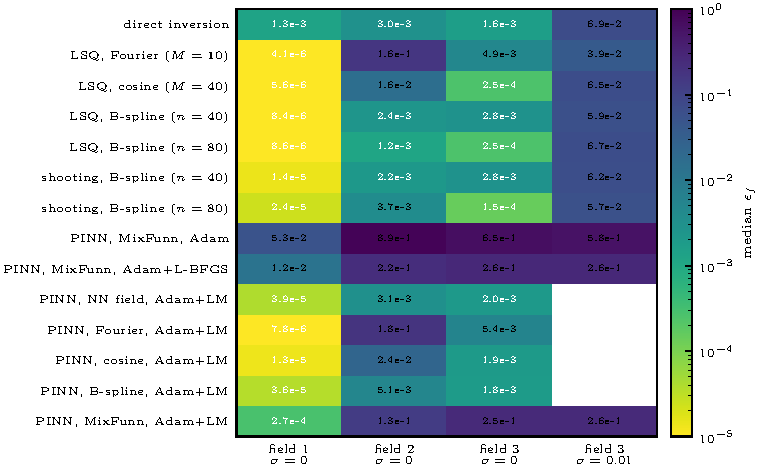
\includegraphics[width=0.62\linewidth]{figS3_overview.pdf}
  \caption{Median field error $\ef$ over five seeds for every method and scenario (current protocol).}
  \label{fig:S3}
\end{figure}

\paragraph{Optimizers.} Table~\ref{tab:optim} lists the field error for field~3 after each second-stage
optimizer (earlier protocol; Fig.~5 of the main text).

\begin{table}[h]
  \caption{Field~3, no noise: relative field error after 3000 Adam steps and each second stage (median
  and range over five seeds; earlier protocol, see Sec.~\ref{sec:protocol}).}
  \label{tab:optim}
  \begin{tabular}{lcccc}
\toprule
second stage & \multicolumn{2}{c}{NN field} & \multicolumn{2}{c}{B-spline field} \\
\cmidrule(lr){2-3}\cmidrule(lr){4-5}
 & $\epsilon_f$ median & [min, max] & $\epsilon_f$ median & [min, max] \\
\midrule
none (Adam only) & $0.26$ & [$0.25$, $0.26$] & $0.25$ & [$0.25$, $0.27$] \\
L-BFGS & $3.3\times10^{-2}$ & [$3.1\times10^{-2}$, $4.4\times10^{-2}$] & $2.5\times10^{-2}$ & [$1.4\times10^{-2}$, $5.9\times10^{-2}$] \\
self-scaled BFGS & $0.10$ & [$7.4\times10^{-2}$, $0.15$] & $9.9\times10^{-2}$ & [$4.7\times10^{-2}$, $0.16$] \\
dense BFGS & $1.3\times10^{-2}$ & [$6.7\times10^{-3}$, $1.7\times10^{-2}$] & $1.1\times10^{-2}$ & [$8.7\times10^{-3}$, $2.3\times10^{-2}$] \\
LM, causal weights in Adam & $1.7\times10^{-3}$ & [$8.9\times10^{-4}$, $2.0\times10^{-3}$] & $7.2\times10^{-3}$ & [$5.2\times10^{-3}$, $8.4\times10^{-3}$] \\
LM & $1.0\times10^{-3}$ & [$9.2\times10^{-4}$, $2.1\times10^{-3}$] & $7.6\times10^{-3}$ & [$5.4\times10^{-3}$, $9.3\times10^{-3}$] \\
\bottomrule
\end{tabular}

\end{table}

\paragraph{Per-scenario results.} Tables~\ref{tab:S_f1}--\ref{tab:S_f3n} and
Figs.~\ref{fig:S4}--\ref{fig:S7} give both metrics, their range over seeds and the mean run time for every
method.

\begin{table}[h]
  \caption{Field~1, no noise.}
  \label{tab:S_f1}
  \begin{tabular}{lcccc}
\toprule
method & $\epsilon_f$ median & $\epsilon_f$ [min, max] & $\epsilon_r$ median & time (s) \\
\midrule
LSQ, Fourier ($M{=}10$) & $4.1\times10^{-6}$ & [$4.1\times10^{-6}$, $4.1\times10^{-6}$] & $5.5\times10^{-7}$ & 0 \\
LSQ, cosine ($M{=}40$) & $5.6\times10^{-6}$ & [$5.6\times10^{-6}$, $5.6\times10^{-6}$] & $5.1\times10^{-7}$ & 0 \\
Fourier ($M{=}10$), Adam + LM & $7.8\times10^{-6}$ & [$2.0\times10^{-6}$, $1.6\times10^{-5}$] & $5.0\times10^{-7}$ & 311 \\
LSQ, B-spline ($n{=}40$) & $8.4\times10^{-6}$ & [$8.4\times10^{-6}$, $8.4\times10^{-6}$] & $6.0\times10^{-7}$ & 0 \\
LSQ, B-spline ($n{=}80$) & $8.6\times10^{-6}$ & [$8.6\times10^{-6}$, $8.6\times10^{-6}$] & $6.9\times10^{-7}$ & 0 \\
cosine ($M{=}40$), Adam + LM & $1.3\times10^{-5}$ & [$8.5\times10^{-6}$, $2.3\times10^{-5}$] & $6.0\times10^{-7}$ & 314 \\
shooting, B-spline ($n{=}40$) & $1.4\times10^{-5}$ & [$1.4\times10^{-5}$, $1.4\times10^{-5}$] & $1.4\times10^{-7}$ & 0 \\
shooting, B-spline ($n{=}80$) & $2.4\times10^{-5}$ & [$2.4\times10^{-5}$, $2.4\times10^{-5}$] & $9.4\times10^{-7}$ & 0 \\
B-spline ($n{=}80$), Adam + LM & $3.6\times10^{-5}$ & [$9.7\times10^{-6}$, $5.9\times10^{-5}$] & $6.7\times10^{-7}$ & 318 \\
NN field, Adam + LM & $3.9\times10^{-5}$ & [$2.3\times10^{-5}$, $4.8\times10^{-5}$] & $8.9\times10^{-7}$ & 288 \\
MixFunn, Adam + LM & $2.7\times10^{-4}$ & [$1.7\times10^{-4}$, $7.9\times10^{-4}$] & $1.5\times10^{-5}$ & 422 \\
direct inversion & $1.3\times10^{-3}$ & [$1.3\times10^{-3}$, $1.3\times10^{-3}$] & $1.2\times10^{-3}$ & 0 \\
MixFunn, Adam + L-BFGS & $1.2\times10^{-2}$ & [$1.1\times10^{-2}$, $2.7\times10^{-2}$] & $6.9\times10^{-4}$ & 55 \\
MixFunn, Adam only & $5.3\times10^{-2}$ & [$3.2\times10^{-2}$, $0.35$] & $8.8\times10^{-3}$ & 80 \\
\bottomrule
\end{tabular}

\end{table}

\begin{figure}[h]
  \centering
  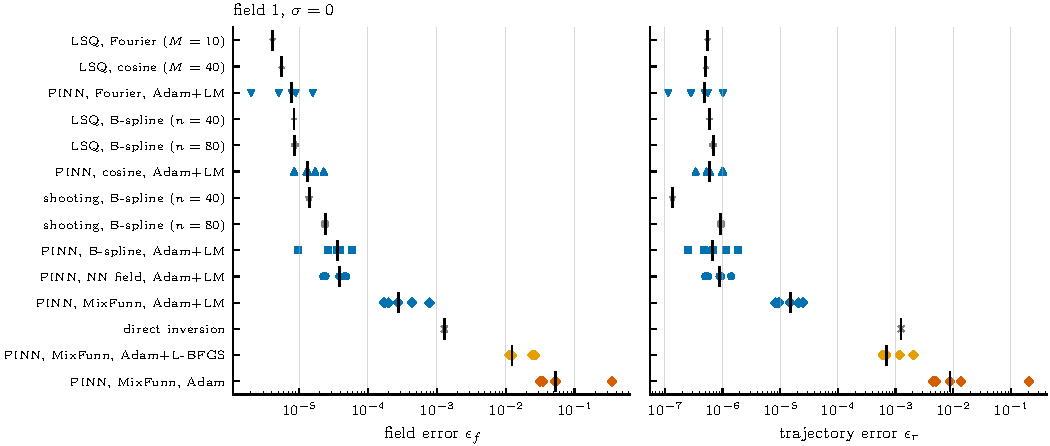
\includegraphics[width=\linewidth]{figS4_detail_field1_noise0.pdf}
  \caption{Field~1, no noise: field error and trajectory error of every run (points) and their medians
  (bars). Colour: optimizer; marker: field representation.}
  \label{fig:S4}
\end{figure}

\begin{table}[h]
  \caption{Field~2, no noise.}
  \label{tab:S_f2}
  \begin{tabular}{lcccc}
\toprule
method & $\epsilon_f$ median & $\epsilon_f$ [min, max] & $\epsilon_r$ median & time (s) \\
\midrule
LSQ, B-spline ($n{=}80$) & $1.2\times10^{-3}$ & [$1.2\times10^{-3}$, $1.2\times10^{-3}$] & $6.2\times10^{-5}$ & 0 \\
shooting, B-spline ($n{=}40$) & $2.2\times10^{-3}$ & [$2.2\times10^{-3}$, $2.2\times10^{-3}$] & $5.9\times10^{-5}$ & 0 \\
LSQ, B-spline ($n{=}40$) & $2.4\times10^{-3}$ & [$2.4\times10^{-3}$, $2.4\times10^{-3}$] & $1.6\times10^{-4}$ & 0 \\
direct inversion & $3.0\times10^{-3}$ & [$3.0\times10^{-3}$, $3.0\times10^{-3}$] & $1.7\times10^{-3}$ & 0 \\
NN field, Adam + LM & $3.1\times10^{-3}$ & [$1.6\times10^{-3}$, $5.1\times10^{-3}$] & $1.1\times10^{-4}$ & 290 \\
shooting, B-spline ($n{=}80$) & $3.7\times10^{-3}$ & [$3.7\times10^{-3}$, $3.7\times10^{-3}$] & $1.5\times10^{-4}$ & 0 \\
B-spline ($n{=}80$), Adam + LM & $5.1\times10^{-3}$ & [$4.5\times10^{-3}$, $1.5\times10^{-2}$] & $2.2\times10^{-4}$ & 319 \\
LSQ, cosine ($M{=}40$) & $1.6\times10^{-2}$ & [$1.6\times10^{-2}$, $1.6\times10^{-2}$] & $4.4\times10^{-3}$ & 0 \\
cosine ($M{=}40$), Adam + LM & $2.4\times10^{-2}$ & [$2.2\times10^{-2}$, $2.8\times10^{-2}$] & $6.7\times10^{-4}$ & 313 \\
MixFunn, Adam + LM & $0.13$ & [$4.8\times10^{-2}$, $0.18$] & $1.0\times10^{-2}$ & 422 \\
LSQ, Fourier ($M{=}10$) & $0.16$ & [$0.16$, $0.16$] & $5.5\times10^{-2}$ & 0 \\
Fourier ($M{=}10$), Adam + LM & $0.18$ & [$0.18$, $0.18$] & $1.0\times10^{-2}$ & 309 \\
MixFunn, Adam + L-BFGS & $0.22$ & [$0.21$, $0.33$] & $1.8\times10^{-2}$ & 51 \\
MixFunn, Adam only & $0.89$ & [$0.32$, $72$] & $0.29$ & 77 \\
\bottomrule
\end{tabular}

\end{table}

\begin{figure}[h]
  \centering
  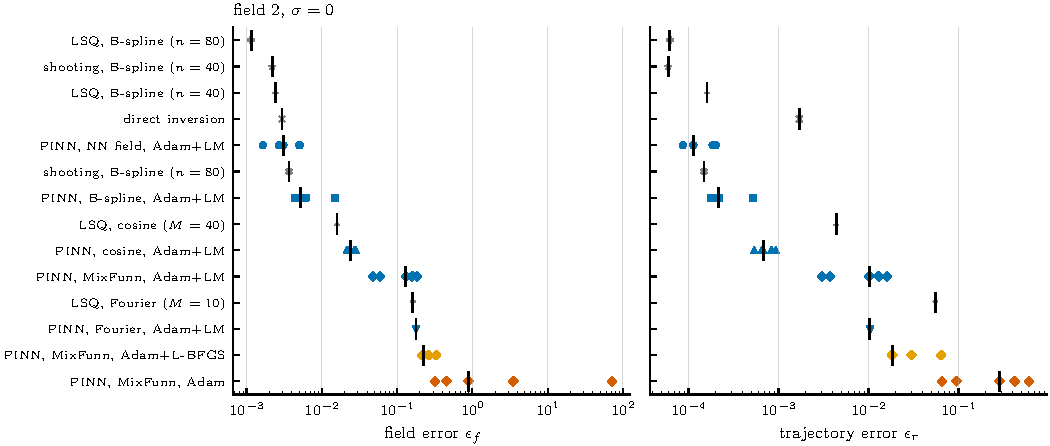
\includegraphics[width=\linewidth]{figS5_detail_field2_noise0.pdf}
  \caption{Field~2, no noise; as Fig.~\ref{fig:S4}.}
  \label{fig:S5}
\end{figure}

\begin{table}[h]
  \caption{Field~3, no noise.}
  \label{tab:S_f3}
  \begin{tabular}{lcccc}
\toprule
method & $\epsilon_f$ median & $\epsilon_f$ [min, max] & $\epsilon_r$ median & time (s) \\
\midrule
shooting, B-spline ($n{=}80$) & $1.5\times10^{-4}$ & [$1.5\times10^{-4}$, $1.5\times10^{-4}$] & $4.1\times10^{-6}$ & 0 \\
LSQ, cosine ($M{=}40$) & $2.5\times10^{-4}$ & [$2.5\times10^{-4}$, $2.5\times10^{-4}$] & $2.6\times10^{-5}$ & 0 \\
LSQ, B-spline ($n{=}80$) & $2.5\times10^{-4}$ & [$2.5\times10^{-4}$, $2.5\times10^{-4}$] & $1.7\times10^{-5}$ & 0 \\
direct inversion & $1.6\times10^{-3}$ & [$1.6\times10^{-3}$, $1.6\times10^{-3}$] & $4.7\times10^{-4}$ & 0 \\
B-spline ($n{=}80$), Adam + LM & $1.8\times10^{-3}$ & [$1.0\times10^{-3}$, $2.0\times10^{-3}$] & $4.2\times10^{-5}$ & 313 \\
cosine ($M{=}40$), Adam + LM & $1.9\times10^{-3}$ & [$1.1\times10^{-3}$, $2.2\times10^{-3}$] & $4.9\times10^{-5}$ & 307 \\
NN field, Adam + LM & $2.0\times10^{-3}$ & [$9.3\times10^{-4}$, $2.2\times10^{-3}$] & $5.8\times10^{-5}$ & 287 \\
shooting, B-spline ($n{=}40$) & $2.8\times10^{-3}$ & [$2.8\times10^{-3}$, $2.8\times10^{-3}$] & $4.2\times10^{-5}$ & 0 \\
LSQ, B-spline ($n{=}40$) & $2.8\times10^{-3}$ & [$2.8\times10^{-3}$, $2.8\times10^{-3}$] & $4.6\times10^{-5}$ & 0 \\
LSQ, Fourier ($M{=}10$) & $4.9\times10^{-3}$ & [$4.9\times10^{-3}$, $4.9\times10^{-3}$] & $4.6\times10^{-4}$ & 0 \\
Fourier ($M{=}10$), Adam + LM & $5.4\times10^{-3}$ & [$5.4\times10^{-3}$, $5.5\times10^{-3}$] & $2.6\times10^{-4}$ & 299 \\
MixFunn, Adam + LM & $0.25$ & [$0.17$, $0.25$] & $1.2\times10^{-2}$ & 422 \\
MixFunn, Adam + L-BFGS & $0.26$ & [$0.25$, $0.26$] & $1.3\times10^{-2}$ & 73 \\
MixFunn, Adam only & $0.65$ & [$0.32$, $55$] & $0.16$ & 82 \\
\bottomrule
\end{tabular}

\end{table}

\begin{figure}[h]
  \centering
  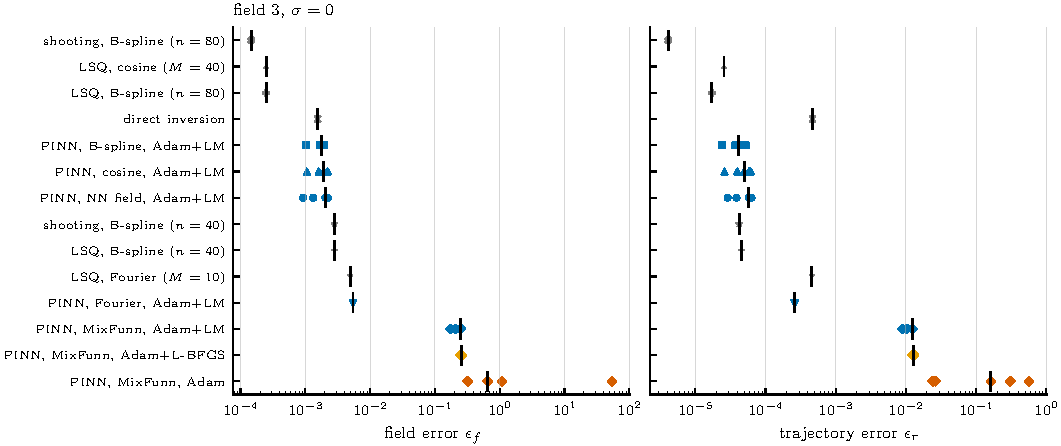
\includegraphics[width=\linewidth]{figS6_detail_field3_noise0.pdf}
  \caption{Field~3, no noise; as Fig.~\ref{fig:S4}.}
  \label{fig:S6}
\end{figure}

\begin{table}[h]
  \caption{Field~3, noise $\sigma=0.01$.}
  \label{tab:S_f3n}
  \begin{tabular}{lcccc}
\toprule
method & $\epsilon_f$ median & $\epsilon_f$ [min, max] & $\epsilon_r$ median & time (s) \\
\midrule
LSQ, Fourier ($M{=}10$) & $3.9\times10^{-2}$ & [$2.9\times10^{-2}$, $5.3\times10^{-2}$] & $4.6\times10^{-3}$ & 0 \\
shooting, B-spline ($n{=}80$) & $5.7\times10^{-2}$ & [$4.8\times10^{-2}$, $9.6\times10^{-2}$] & $2.9\times10^{-3}$ & 1 \\
LSQ, B-spline ($n{=}40$) & $5.9\times10^{-2}$ & [$5.6\times10^{-2}$, $6.7\times10^{-2}$] & $5.0\times10^{-3}$ & 0 \\
shooting, B-spline ($n{=}40$) & $6.2\times10^{-2}$ & [$5.4\times10^{-2}$, $0.11$] & $3.1\times10^{-3}$ & 0 \\
LSQ, cosine ($M{=}40$) & $6.5\times10^{-2}$ & [$6.1\times10^{-2}$, $7.2\times10^{-2}$] & $4.9\times10^{-3}$ & 0 \\
LSQ, B-spline ($n{=}80$) & $6.7\times10^{-2}$ & [$6.5\times10^{-2}$, $7.2\times10^{-2}$] & $5.0\times10^{-3}$ & 0 \\
direct inversion & $6.9\times10^{-2}$ & [$6.8\times10^{-2}$, $7.5\times10^{-2}$] & $4.9\times10^{-3}$ & 0 \\
MixFunn, Adam + LM & $0.26$ & [$4.8\times10^{-2}$, $0.26$] & $1.3\times10^{-2}$ & 423 \\
MixFunn, Adam + L-BFGS & $0.26$ & [$0.24$, $0.27$] & $1.3\times10^{-2}$ & 119 \\
MixFunn, Adam only & $0.58$ & [$0.31$, $1.2$] & $0.13$ & 140 \\
\bottomrule
\end{tabular}

\end{table}

\begin{figure}[h]
  \centering
  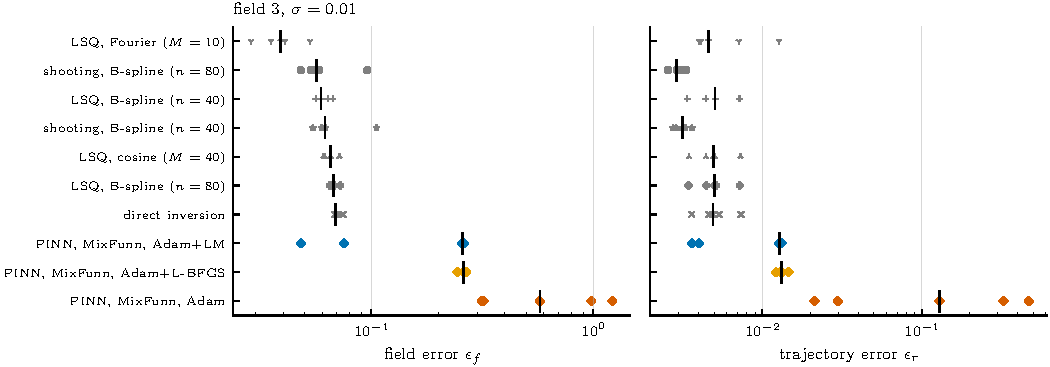
\includegraphics[width=\linewidth]{figS7_detail_field3_noise0p01.pdf}
  \caption{Field~3, noise $\sigma=0.01$; as Fig.~\ref{fig:S4}.}
  \label{fig:S7}
\end{figure}

\clearpage
% =====================================================================================
\section{Outlook settings: details}\label{sec:outlook}

\paragraph{Two-qubit model.} The two-qubit notebooks of the repository
(\texttt{notebooks/modelo\_2(Rede neural)/PINN\_field\_4\_twoqubits\_*.ipynb}) use
\begin{equation}
  H(t)=\omega_2\,\sigma_z\otimes\mathbb 1+\omega_1\,\mathbb 1\otimes\sigma_z
       +f(t)\,(\sigma_x\otimes\sigma_x+\sigma_y\otimes\sigma_y),
\end{equation}
with $\omega_1=\omega_2=0.5$, field~3 with $T=2\pi$, $N=200$ time points, initial state
$|{+}\rangle|{+}\rangle$, the fifteen observables $\langle\sigma_\mu\otimes\sigma_\nu\rangle$
($(\mu,\nu)\ne(0,0)$), and, in the open case, Lindblad operators $\sqrt{\gamma}\,\sigma_\pm$ on each qubit
with $\gamma=0.05$~\cite{lindblad1976,gorini1976}. The expectation values obey
$\frac{d}{dt}\langle S\rangle=i\langle[H,S]\rangle+\sum_k\gamma_k\langle\mathcal L_k^{\dagger}S\mathcal L_k
-\tfrac12\{S,\mathcal L_k^{\dagger}\mathcal L_k\}\rangle$, the form used in the PINNverse
framework~\cite{castelano2024freezing,delima2025pinnverse}.

\paragraph{Blind states and phase dependence.} We checked numerically (QuTiP, tolerance $10^{-12}$) that
(i)~starting from $|00\rangle$, the fifteen expectation values for $f$ and $f/2$ coincide exactly, both
for $\omega_1=\omega_2=0.5$ and for $\omega_1=0.5$, $\omega_2=0.7$, whereas from $|01\rangle$ and
$|{+}{+}\rangle$ they differ by up to $1.7$ and $0.97$; and (ii)~for $\omega_1=\omega_2$, where
$\|[H_0,H_1]\|=0$, the expectation values equal those of $e^{-iH_0t}e^{-i\Phi(t)H_1}|{+}{+}\rangle$
with $\Phi(t)=\int_0^tf$ to $1.7\times10^{-7}$. The data therefore determine $\Phi(t)$, and $f=\dot\Phi$.

\paragraph{Partial information.} With only $\langle\sigma_z\rangle$ measured, the PINN loss keeps the full
Bloch equations for $(X,Y,Z)$ and restricts the data term to $Z$; shooting restricts its residual to $Z$;
direct inversion and LSQ are not applicable. The symmetries of Sec.~\ref{sec:identifiability} require an
initial state with $X,Y,Z$ all nonzero, or two measured components. The planned extension of the
protocol is described in \texttt{notes/TODO.md} of the repository.

\bibliographystyle{apsrev4-2}
\bibliography{references}

\end{document}
